\documentclass[11pt, oneside]{article}   	% use "amsart" instead of "article" for AMSLaTeX format
\usepackage{geometry}                		% See geometry.pdf to learn the layout options. There are lots.
\geometry{letterpaper}                   		% ... or a4paper or a5paper or ... 
%\geometry{landscape}                		% Activate for for rotated page geometry
%\usepackage[parfill]{parskip}    		% Activate to begin paragraphs with an empty line rather than an indent
\usepackage{graphicx}				% Use pdf, png, jpg, or eps� with pdflatex; use eps in DVI mode
								% TeX will automatically convert eps --> pdf in pdflatex		
\usepackage{amssymb}
\usepackage{amsmath}

\title{Auroux Ch. 23:  Flux}
%\author{The Author}
\date{}							% Activate to display a given date or no date

\graphicspath{{/Users/telliott_admin/Dropbox/Tex/png/}}
\begin{document}
\maketitle
%\section{}
% \subsection*{R code}
% \begin{lstlisting}  \end{lstlisting}
% \begin{center} 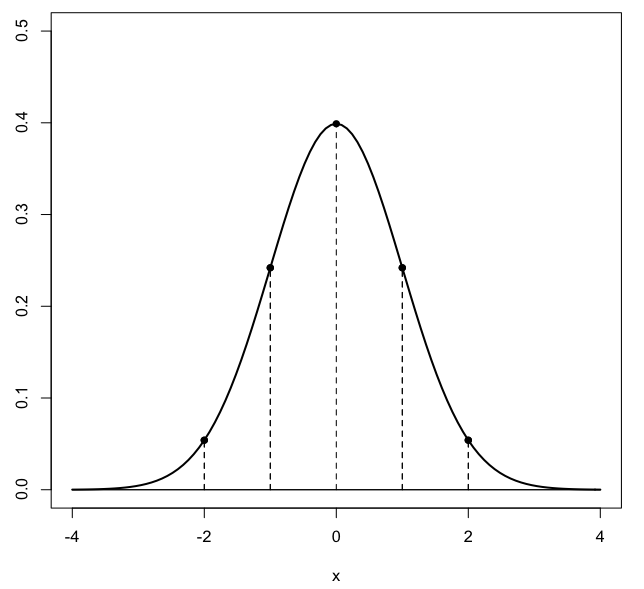
\includegraphics [scale=0.4] {gauss3.png} \end{center}
% \begin{bmatrix} a  &  b \\ c  &  d \end{bmatrix}
% \bigg |_

\large
\noindent
To review, we compute work as
\[ W = \int_C \mathbf{F} \cdot d\mathbf{r} \]
As a shorthand we say that
\[ {W = \int_C M dx + N dy} \]
We get from one to the other by deconstructing $d\mathbf{r}$
\[ d\mathbf{r} = \hat{\mathbf{T}} \ ds = \frac{d\mathbf{r}}{dt} \ dt \]
where
\[ \frac{d\mathbf{r}}{dt} = \ <\frac{dx}{dt},\frac{dy}{dt}> \]
Hence, if we have $\mathbf{F} = <M,N>$ then
\[ W = \int_C \mathbf{F} \cdot \frac{d\mathbf{r}}{dt} \ dt = \int_C <M,N> \cdot <\frac{dx}{dt},\frac{dy}{dt}> \ dt = \int_C M dx + N dy \]
\subsection*{example}
If 
\[ \mathbf{F} = <-y,x> \]
\[ x = t, \ \ y = t^2 \]
we obtain
\[ W = \int_C <M,N> \cdot <\frac{dx}{dt},\frac{dy}{dt}> \ dt \]
\[ = \int_C <-t^2,t> \cdot < 1,2t> \ dt \]
\[ = \int_C t^2 \]
\[ = \frac{1}{3}t^3 \ \bigg |_{P1}^{P2}  \]

\subsection*{Flux}
In this write-up, we're concerned with Flux, which also has a shorthand
\[ Flux = \int_C -N dx + M dy \]
We switched $M$ for $N$ and changed signs.

Work is done by the component of the force in the direction of $\hat{\mathbf{T}}$.  It's the "tail wind", if you will.  Flux is the "cross-wind", it is the component $\perp \hat{\mathbf{T}}$.
\[ Flux = \int_C \mathbf{F} \cdot \hat{\mathbf{n}} \ ds \]
We'll show a derivation below.
\subsection*{Example}
Sometimes we don't need to calculate!  Suppose 
\[ \mathbf{F} = \ <x,y> \]
a radial field.  Let $C$ be a circle of radius $a$ centered at the origin.  In this situation the formula with $\hat{\mathbf{n}}$ is useful.
\[ \mathbf{F}  \cdot \hat{\mathbf{n}} = |F| |n| cos \theta = |F| = \sqrt{x^2 + y^2} = a \]
So
\[ Flux = \int_C \mathbf{F} \cdot \hat{\mathbf{n}} \ ds \]
\[ = \int_C a \ ds = a \int_C \ ds \]
\[ = a \ 2\pi a \]
\[ = 2\pi a^2 \]

Note that $\hat{\mathbf{n}}$ is just $\hat{\mathbf{T}}$ rotated by $90^\circ$ cw.  (The convention is that the integral should be positive if we move along the curve with the region on our left).  Now
\[ d \mathbf{r} = \ <dx,dy> \ \]
\[ = \hat{\mathbf{T}} \ ds \]
so
\[ \hat{\mathbf{n}} \ ds = <dy, -dx> \]
and
\[ \int_C \mathbf{F} \cdot \hat{\mathbf{n}} \ ds \]
\[ = \int_C <M,N> \cdot <\frac{dy}{dt},-\frac{dx}{dt}> \ dt \]
which we can try to remember as
\[ = \int_C -N dx + M dy \]
as shown above.
\subsection*{Green's Theorem}
Our statement of the theorem was that
\begin{equation}
  \boxed{ \int_C M dx + N dy = \int \int_R (N_x - M_y) \ dA }
\end{equation}
We can use the "del" notation to make this shorter
\[ \int_C M dx + N dy = \int \int_R (N_x - M_y) \ dA \]
\[ = \int \int_R \nabla \times \mathbf{F} \ dA\]
I will come back to that cross-product in a minute.  But $N_x - M_y$ is the curl of $\mathbf{F}$.
Now we just switch letters!  Put $-N$ for $M$ and $M$ for $N$
\begin{equation}
  \boxed{ \int_C -N dx + M dy = \int \int_R (M_x + N_y) \ dA =  \int \int_R \nabla \cdot \mathbf{F} \ dA}
\end{equation}


This is Green's Theorem for Flux.  The left-hand side is the Flux, the right-hand side is a way to calculate the same quantity using $\nabla \cdot \mathbf{F}$
\subsection*{example}
Suppose $\mathbf{F}= \ <x,y>$ and the curve is a circle of radius $a$, but centered at $(0,2)$.  So now parametrization gets a little trickier..
But notice that
\[ \nabla \cdot \mathbf{F} = 2 \]
So we can calculate the Flux by using Green's Thm (for Flux).  It is just
\[ \int \int_R \nabla \cdot \mathbf{F} \ dA = 2 \int \int_R dA = 2\pi a^2 \]
and this is true regardless of where the circle is.
\subsection*{Notation}
So we have the symbol $\nabla$ which we use as an operator
\[ \nabla = \frac{\partial}{\partial x}, \frac{\partial}{\partial y}, \frac{\partial}{\partial z} \]
We have already used this in defining the \emph{gradient} of $f$
\[ \nabla f = \frac{\partial f}{\partial x}, \frac{\partial f}{\partial y}, \frac{\partial f}{\partial z} = \ < f_x, f_y, f_z > \]
Now we introduce a dot product and cross product employing $\nabla$.  The first is the divergence of $\mathbf{F}$
\[ \mathbf{F} = \ <P,Q,R> \]
\[ \nabla \cdot \mathbf{F} = P_x + Q_y + R_z \]
And the second is the curl of $\mathbf{F}$
\[ \nabla \times \mathbf{F} \]

\[
\begin{vmatrix} 
  \hat{i}  &  \hat{j} & \hat{k} \\ 
  \frac{\partial}{\partial x}  &  \frac{\partial}{\partial y} & \frac{\partial}{\partial z} \\ 
  P  &  Q & R \\ 
\end{vmatrix} \ \ 
\]
This determinant has three components
\[ | (\frac{\partial R}{\partial y} - \frac{\partial Q}{\partial z}) - (\frac{\partial R}{\partial x} - \frac{\partial P}{\partial z}) +
(\frac{\partial Q}{\partial x} - \frac{\partial P}{\partial y}) |
\]
What we have in Green's Theorem (with different letters, substitute N for Q and M for P), is a vector with only $x$ and $y$ components and hence only one of the terms.

\end{document}  